\documentclass[pdftex,11pt]{article}

\usepackage{times}
\usepackage{fullpage}
\usepackage{natbib}
\usepackage{url}
\usepackage{latexsym}
\usepackage[pdftex]{graphicx} \pdfcompresslevel=9

\usepackage{algpseudocode}

\usepackage{amsmath}
\DeclareMathOperator*{\argmax}{arg\,max}

\usepackage{array}
\usepackage{multirow}
\usepackage[utf8x]{inputenc}

% \usepackage[font=footnotesize]{subfig}
\usepackage{url}

\usepackage{color}
\newcommand{\Note}[1]{\textcolor{blue}{\small [#1]}}
% \newcommand{\Note}[1]{}
%\usepackage{draftwatermark}

\hyphenation{net-works}

\begin{document}

\title{Detecting and Modeling Text Reuse in Nineteenth-Century Newspapers}

\author{Ryan Cordell \and David A. Smith \and Elizabeth Maddock Dillon}

\date{}

\maketitle


\begin{abstract}
  Texts propagate through many social networks and provide evidence
  for their structure.  We present efficient algorithms for detecting
  clusters of reused passages embedded within longer documents in
  large collections.  We apply these techniques to analyzing the
  culture of reprinting in the United States before the Civil War.
  Without substantial copyright enforcement, stories, poems, news, and
  anecdotes circulated freely among newspapers, magazines, and books.
  From a collection of OCR'd newspapers, we extract a new corpus of
  reprinted texts, explore the geographic spread and network
  connections of different publications, and analyze the time dynamics
  of different genres.
\end{abstract}

\section{Introduction}
\label{sec:intro}

Many studies of social networks and interactions use surveys and
observational data on nodes and links.  This metadata is often
augmented by the language the members of a social network use to
interact with each other---e.g., the text of email messages within a
company or of posts and tweets exchanged among online social network
participants.  In some cases, however, we cannot directly observe
network links, or even get a census of network nodes, and yet we can
still observe text that provides evidence for social interactions.

A particularly useful form of evidence comes from copying and
quotation of text by different actors in a social network.  The social
ties indicated by text reuse may be overt, as with acknowledged
quotations of earlier scholarly work, or unacknowledged, as with
legislators' adoption, when drafting bills, of language from interest
groups' policy documents.  In aggregate, text reuse patterns can
provide evidence for direct or indirect contact between different
social actors.  Examination of the reused passages can provide
evidence for the shared interests of groups.  At a finer level of
analysis, the temporal and spatial dynamics of text reuse can provide
evidence for individual links and propagation patterns in networks
\cite{leskovec09:_meme_dynam_news_cycle,lease12:_findin_explor_memes_social_media}.

Our approach to local text reuse detection and clustering is motivated
by the analysis of a corpus of nineteenth century U.S. newspapers to
investigate the ``culture of reprinting'' that existed before
effective copyright enforcement and wire services.  While this paper
focuses on the textual evidence alone, a more general setup could
employ both text and information about some \emph{related} network.
\citet{namata11:_collec_graph_ident}, for instance, considered the
task of inferring corporate hierarchies from the network of email
communications.  In the case study on 19c newspapers, we might use the
railroad and telegraph networks as additional evidence for how news
and culture propagated.

Researchers in NLP and information retrieval have often employed text
reuse detection to remove duplicates from web crawls and search
results and to detect plagiarism in documents and source code.  These
methods can achieve quite high precision when the majority of
documents' contents are implicated in reuse.  Performance is often
tuned for ad-hoc retrieval, with one or a few query documents (e.g.,
student submissions) being run against a large corpus of potential
matches.  We are interested, however, in the overall patterns of text
reuse and focus here on a different task: near-neighbor search among
all document pairs for overlapping passages.  For a web crawler, lower
recall simply leads to a larger index; in our case, low recall on the
text reuse task can lead to inaccurate output.

At a high level, the method proposed in this paper (1) finds pairs of
documents likely to contain substantial overlap, (2) performs an
alignment to find passages of local similarity even if the rest of the
documents are unrelated, and (3) uses that pairwise passage
information to infer larger clusters of text reuse.  As we explain in
more detail below, there are two primary sources of error in this
process, in addition to the appearance of resemblance arising by
chance that affects other work on sequence similarity from NLP to
bioinformatics.  First, since our collections contain multiple
documents from the same source, precision can be hurt by often
substantial amounts of intra-source text reuse, which are not as
important when looking for evidence of interaction among sources.
Second, since we are often interested in mapping networks in
historical data, text that has been poorly transcribed by optical
character recognition can depress recall.

Our approach, like many others, involves ``shingling''---evaluating
document pairs by the intersection of their n-gram features---, but
these considerations require further refinements to optimize
effectiveness and efficiency.  In particular, we employ hashing for
space-efficient indexing of repeated n-grams and the use of
overlapping n-grams to prune dynamic programming for local alignment.

Before describing methods for detecting and clustering passages of
local text reuse in \S\ref{sec:detection}, we provide background on
reprinting in 19c newspapers in order to motivate some of our design
choices (\S\ref{sec:tracking-newspapers}).  In \S\ref{sec:evaluation}, we
describe experimental evaluations of the effectiveness and efficiency
of various text reuse detection approaches and of the ability of text
reuse approaches to detect actual policy borrowing in legislative
bills.  Finally, we investigate interesting properties of the most
popular texts, explore the geographic spread and network connections
of different texts and publications, analyze some of the text reuse
dynamics of different genres of texts, and measure the accuracy for
reprint prediction of different newspaper attributes
(\S\ref{sec:eda}).

\section{Tracking Viral Texts in 19c Newspapers}
\label{sec:tracking-newspapers}

In \emph{American Literature and the Culture of Reprinting},
\citet{mcgill03:_americ_liter_cultur_reprin} argues that American
literary culture in the nineteenth century was shaped by the
widespread practice of reprinting stories and poems, usually without
authorial permission or even knowledge, in newspapers, magazines, and
books.  Without substantial copyright enforcement, texts circulated
promiscuously through the print market and were often revised by
editors during the process.  These ``viral'' texts---be they news
stories, short fiction, or poetry---are much more than historical
curiosities.  The texts that editors chose to pass on are useful
barometers of what was exciting or important to readers during the
period, and thus offer significant insight into the priorities and
concerns of the culture.  Nineteenth-century U.S. newspapers were
usually associated with a particular political party, religious
denomination, or social cause (e.g., temperance or abolition).
Mapping the specific locations and venues in which varied texts
circulated would therefore allow us to answer questions about how
reprinting and the public sphere in general were affected by
geography, communication and transportation networks, and social,
political, and religious affinities.

To study the reprint culture of this period, we crawled the online
newspaper archives of the Library of Congress's \emph{Chronicling
  America} project (\url{chroniclingamerica.loc.gov}).  Since the
Chronicling America project aggregates state-level digitization
efforts, there are some significant gaps: e.g., there are no
newspapers from Massachusetts, which played a not insubstantial role
in the literary culture of the period.  While we continue to collect
data from other sources in order to improve our network analysis, the
current dataset remains a useful, and open, testbed for text reuse
detection and analysis of overall trends.

Another difficulty with this collection is that it consists of the
OCR'd text of newspaper issues without any marking of article breaks,
headlines, or other structure.  The local alignment methods described
in \S\ref{sec:alignment} are designed not only to mitigate this
problem, but also to deal with partial reprinting.  One newspaper
issue, for instance, might reprint chapters 4 and 5 of a Thackeray
novel while another issue prints only chapter 5.

Since our goal is to detect texts that spread from one venue to
another, we are not interested in texts that were reprinted frequently
in the same newspaper, or \textit{series}, to use the cataloguing
term.  This includes material such as mastheads and manifestos and
also the large number of advertisements that recur week after week in
the same newspaper.

The methods we discuss in this paper could also be applied, of course,
to other domains.  Most closely related to previous work on plagiarism
detection is the investigation in historical and literary studies of
the sources that influenced a text, sometimes referred to as
\emph{source criticism}.

\section{Text Reuse Detection}
\label{sec:detection}

As noted above, we are interested in detecting passages of text reuse
(individual articles) that comprise a very small fraction of the
containing documents (newspaper issues).  Using the terminology of
biological sequence alignment, we are interested in \emph{local
  alignments} between documents.
\citet{henzinger06:_findin_near_duplic_web_pages} provides a good
overview of text reuse detection research and provides an empirical
evaluation of the two primary methods---n-gram shingling and
locality-sensitive hashing (LSH)---on near-duplicate webpage detection
tasks.  The need for local alignments makes LSH less practical without
performing a large number of sliding-window matches.\footnote{While
  there is some work on embedding string edit distances for LSH, it
  applies to measures of \emph{global} alignment such as Hamming
  distance and cyclic shifts \cite{andoni13:_homom_finger_misal}.} We
therefore base our approach on n-gram shingling.

Several attributes distinguish the present approach from previous
work:
\begin{itemize}

\item The boundaries of the reused passages are not known, in contrast
  to near-duplicate document detection and to work on ``meme
  tracking'' that takes text between quotation marks as the unit of
  reuse \cite{leskovec09:_meme_dynam_news_cycle,suen13:nifty}.

\item Also in contrast to this work on the contemporary news cycle and
  blogosphere, we are interested both in texts that are reprinted
  within a few days and after many years.  We thus cannot exclude
  potentially matching documents for being far removed in time.

\item We are looking for reuse of substantial amounts of text, on the
  order of 100 words or more, in contrast to work on detecting shorter
  quotations
  \cite{kolak08:_gener_links_minin_quotat,seo08:_local_text_reuse_detec,horton10:_somet_borrow,lease12:_findin_explor_memes_social_media}.

\item We wish to compute all nearest neighbor passages, instead of
  running a small number of query documents against a corpus.

\item Text reuse that occurs only among documents from the same
  ``source'' should be excluded.
  \citet{henzinger06:_findin_near_duplic_web_pages} notes, for
  instance, that many of the errors in near-duplicate webpage
  detection arose from false matches among documents from the same
  website that shared boilerplate navigational elements.

\item We require methods that are robust to noisy OCR transcripts.
  While we could adopt a pipelined approach and perform OCR correction
  before text reuse detection, it is worth noting that a promising
  source of data for OCR correction are the clusters of similar
  passages found in other documents.

\end{itemize}

In common with work in duplicate detection, we start the search for
reused passages by first finding likely document pairs.  For each
document pair returned by this first step, we then identify a passage
embedded within each document that is a good local match for the
other.  We then greedily aggregate this pairwise data into large
clusters of reused text passages.  We now describe the details of each
step in turn.

\subsection{Search for Candidate Document Pairs}
\label{sec:all-pairs}

We begin with a scan for document pairs likely to contain reprinted
passages.  We use ``shingling'', which represents documents by an
unordered collection of its n-grams, to provide features for document
similarity computations.  We balance recall and precision by adjusting
the size of the shingles and the proportion of the shingles that are
used to calculate document similarity.  After determining which
features will be used to represent documents, we build an index of the
repeated n-grams and then extract candidate document pairs from this
index.  Table~\ref{tab:parameters} shows the parameters used in our
approach.

\subsubsection{N-gram Document Representations}
\label{sec:ngrams}

The choice of document representation affects the precision and
recall, as well as the time and space complexity of a text reuse
detection system.  In our experiments, we adopt the popular choice of
n-grams, contiguous subsequences of $n$ words.  Very similar passages
of sufficient length will share many long subsequences, but long
n-grams are less robust to textual variation and OCR errors.  As we
see in the experiments below (\S\ref{sec:evaluation}), values of $n$
between 5 and 7 provide a reasonable tradeoff between accuracy and
efficiency for the newspaper corpus while longer n-grams work well on
the cleaner legislative corpus.

In previous work on detecting short quotes or ``memes'', short
contiguous n-grams have been proven to be quite effective.
\citet{suen13:nifty}, for instance, use 4-grams to identify similar
quotes in newspaper articles and blogs.  Many fixed phrases, however,
will also be detected by that approach.  For instance, two documents
are not much more likely to be derived from the same source if they
both include the 5-grams ``it is no accident that'' and ``in the final
analysis it''.  We will see how to mitigate this problem by upper
bounding the document frequency of the n-grams we use.

In addition to standard contiguous n-grams, therefore, we also
explored the use of \emph{skip n-grams}, or non-contiguous
subsequences of the document.  Skip n-grams allow us to look at
subsequences of words that fall in more widely separate parts of the
document.  We parameterized our skip n-grams by $n$, the number of
terms included; $g$, the minimum gap between terms; and $w$, the
maximum number of terms covered by the skip n-gram.  A contiguous
5-gram would thus be $n$=5 $g$=1 $w$=5.  In this paper, we confine
ourselves to skip bigrams ($n$=2) with width up to 105.

\subsubsection{Downsampling Document Features}
\label{sec:downsampling}

Since duplicate texts will share many matching n-grams, many systems
use only a small fraction of the n-grams to represent each document.

One of the most popular downsampling techniques is 0 mod $p$
\cite{bernstein04:_scalab_system_ident_co_docum}.  When indexing a
document, this technique hashes each n-gram to an integer and then
determines whether the hash value is divisible by some integer $p$.
Since instances of the same n-gram in all documents hash to the same
value, the algorithm does not need to maintain a dictionary of the
downsampled features.  This also permits easy parallelization since
the hash functions can be computed independently in each batch.  Many
duplicate detection systems for the web use $p = 50$ or
above, which drastically reduces index sizes
\cite{henzinger06:_findin_near_duplic_web_pages}.  This downsampling
technique is less effective for local as opposed to global text reuse
\cite{seo08:_local_text_reuse_detec} and can also hurt recall for
noisily OCR'd documents, as we see below.

For bigrams, we also adopt filtering on stopwords.  While indexes of
longer n-grams are not dominated by stopword-only entries, pairs of
stopwords can increase the size of a bigram index significantly.  Due
to the prevalence of OCR errors in the newspaper dataset, we treat all
words of four or fewer characters as stopwords.  Also on the stoplist
are the terms with the highest document frequency that make up $2/3$
of the tokens in the corpus.  On the newspaper collection, leaving out
the four-character-or-less terms, this amounted to 1440 stopwords.  We
ignore any bigram with at least one stopword.  This filter proved to
be too stringent with longer n-grams, though some variants might be
successful.

\subsubsection{Efficient N-gram Indexing}
\label{sec:indexing}

The next step is to build for each n-gram feature an inverted index of
the documents where it appears.  As in other duplicate detection and
text reuse applications, we are only interested in the n-grams shared
by two or more documents.  The index, therefore, does not need to
contain entries for the n-grams that occur only once.  We use the
two-pass space-efficient algorithm described in
\citet{huston11:_effic_index_repeat}, which, empirically, is very
efficient on large collections.  In a first pass, n-grams are hashed
into a fixed number of bins.  On the second pass, n-grams that hash to
bins with one occupant can be discarded; other postings are passed
through.  Due to hash collisions, there may still be a small number of
singleton n-grams that reach this stage.  These singletons are
filtered out as the index is written.

In building an index of n-grams, an index of (n-1)-grams can also
provide a useful filter.  No 5-gram, for example, can occur twice
unless its constituent 4-grams occur at least twice.  We do not use
this optimization in our experiments; in practice, n-gram indexing is
less expensive than the later steps.

\subsubsection{Extracting and Ranking Candidate Pairs}
\label{sec:extracting-pairs}

Once we have an inverted index of the documents that contain each
(skip) n-gram, we use it to generate and rank document pairs that are
candidates for containing reprinted texts.  Each entry, or
\emph{posting list}, in the index may be viewed as a set of pairs
$(d_i, p_i)$ that record the document identifier and position in that
document of that n-gram.

Once we have a posting list of documents containing each distinct
n-gram, we output all pairs of documents in each list.  We suppress
repeated n-grams that appear in different issues of the same
newspaper. These repetitions often occur in editorial boilerplate or
advertisements, which, while interesting, are outside the scope of
this project.  We also suppress n-grams that generate more than $u
\choose 2$ pairs, where $u$ is a parameter.\footnote{The filter is
  parameterized this way because it is applied after removing document
  pairs in the same series.}  These frequent n-grams are likely to be
common fixed phrases.  Filtering terms with high document frequency
has led to significant speed increases with small loss in accuracy in
other document similarity work
\cite{elsayed08:_pairw_docum_simil_large_collec_mapred}.  We then sort
the list of repeated n-grams by document pair, which allows us to
assign a score to each pair based on the number of overlapping n-grams
and the distinctiveness of those n-grams.  When downsampling n-grams
with 0 mod $p$, we use the entire ranked list; otherwise, we confine
our evaluation to document pairs with 5 or more shared n-grams.

\begin{table}
  \centering
  \begin{tabular}{l l} \\
  $n$ & n-gram order \\
  $w$ & maximum width of skip n-grams \\
  $g$ & minimum gap of skip n-grams \\
  $p$ & n-grams downsampled with $0 \mod p$ \\
  $u$ & maximum distinct series in the posting
  list \\
  \end{tabular}
  \caption{Parameters for text reuse detection}
  \label{tab:parameters}
\end{table}

\subsection{Local Document Alignment}
\label{sec:alignment}

The initial pass returns a large ranked list of candidate document
pairs, but it ignores the order of the n-grams as they occur in each
document.  We therefore employ local alignment techniques to find
compact passages with the highest probability of matching.  The goal
of this alignment is to increase the precision of the detected
document pairs while maintaining high recall.  Due to the high rate of
OCR errors, many n-grams in matching articles will contain slight
differences.

Unlike some partial duplicate detection techniques based on global
alignment \cite{yalniz11:_partial_duplic_detec_large_book_collec}, we
cannot expect all or even most of the articles in two newspaper
issues, or the text in two books with a shared quotation, to align.
Rather, as in some work on biological subsequence alignment
\cite{gusfield97:_algor_strin_trees_sequen}, we are looking for
regions of high overlap embedded within sequences that are otherwise
unrelated.  We therefore employ the Smith-Waterman dynamic programming
algorithm with an affine gap penalty.  We use the simplest form of a
weight matrix common in the bioinformatics community: matching
characters have a weight of 2, mismatches have -1, opening a gap is
-5, and continuing a gap is -0.5.  This use of model-based alignment
also distinguishes this approach for other work, for detecting shorter
quotations, that greedily expands areas of n-gram overlap
\cite{kolak08:_gener_links_minin_quotat,horton10:_somet_borrow}.  We
do, however, prune the dynamic programming search by forcing the
alignment to go through position pairs that contain a matching n-gram
from the previous step, as long as the two n-grams are unique in their
respective texts.

Even the exact Smith-Waterman algorithm, however, is an approximation
to the problem we aim to solve.  If, for instance, two separate
articles from one newspaper issue were reprinted in another newspaper
issue in the opposite order---or separated by a long span of unrelated
matter---the local alignment algorithm would simply output the
better-aligned article pair and ignore the other.  Anecdotally, we
only observed this phenomenon once in the newspaper collection, where
two different parodies of the same poem were reprinted in the same
issue.  In any case, our approach can easily align different passages
in the same document to passages in two other documents.
The dynamic program proceeds as follows.  In this paper, two documents
would be treated as sequences of text $X$ and $Y$ whose individual
characters are indexed as $X_i$ and $Y_j$. Let $W(X_i, Y_j)$ be the
score of aligning character $X_i$ to character $Y_j$.  Higher scores
are better.  We use a scoring function where only exact character
matches get a positive score and any other pair gets a negative score.
We also account for additional text appearing on either $X$ or $Y$.
Let $W_g$ be the score, which is negative, of starting a ``gap'',
where one sequence includes text not in the other.  Let $W_c$ be the
cost for continuing a gap for one more character.  This ``affine gap''
model assigns a lower cost to continuing a gap than to starting one,
which has the effect of making the gaps more contiguous.  We use an
assignment of weights fairly standard in genetic sequences where
matching characters score 2, mismatched characters score -1, beginning
a gap costs -5, and continuing a gap costs -0.5.  We leave for future
work the optimization of these weights for the task of capturing
shared policy ideas.

As with other dynamic programming algorithms such as Levenshtein
distance, the Smith-Waterman algorithm operates by filling in a
``chart'' of partial results.  The chart in this case is a set of
cells indexed by the characters in $X$ and $Y$, and we initialize it
as follows:
\begin{align*}
  H(0, 0) & = 0 \\
  H(i, 0) & = E(i, 0) = W_g + i \cdot W_c \\
  H(0, j) & = F(0, j) = W_g + j \cdot W_c
\end{align*}
\noindent The algorithm is then defined by the following recurrence
relations:
\begin{align*}
  H(i, j) & = \max\left\{
    \begin{array}{l}
      0 \\
      E(i, j) \\
      F(i, j) \\
      H(i - 1, j - 1) + W(X_i, Y_j) \\
    \end{array} \right. \\
  E(i, j) & = \max \left\{
    \begin{array}{l}
      E(i, j - 1) + W_c \\
      H(i, j - 1) + W_g + W_c \\
    \end{array} \right. \\
  F(i, j) & = \max \left\{
    \begin{array}{l}
      F(i - 1, j) + W_c \\
      H(i - 1, j) + W_g + W_c \\
    \end{array} \right. \\
\end{align*}

\noindent The main entry in each cell $H(i,j)$ represents the score of
the best alignment that terminates at position $i$ and $j$ in each
sequence.  The intermediate quantities $E$ and $F$ are used for
evaluating gaps.  Due to taking a max with 0, $H(i,j)$ cannot be
negative.  This is what allows Smith-Waterman to ignore text before
and after the locally aligned substrings of each input.

After completing the chart, we then find the optimum alignment by
tracing back from the cell with the highest cumulative value $H(i, j)$
until a cell with a value of 0 is reached. These two cells represent
the bounds of the sequence, and the overall SW alignment score
reflects the extent to which the characters in the sequences align and
the overall length of the sequence.

In our implementation, we include one further speedup: since in a
previous step we identified n-grams that are shared between the two
documents, we assume that any alignment of those documents must include
those n-grams as matches.  In some cases, this anchoring of the
alignment might lead to suboptimal SW alignment scores.

\subsection{Passage Clustering}
\label{sec:clustering}

We now have a set of aligned passage pairs.  We sort the passage pairs
in descending order by length and perform greedy single-link
clustering.  If two passages in the same document overlap by 80\%,
they are taken to be the same passage for purposes of clustering;
otherwise, they are treated as different passages.  Given this
placement of passages into equivalence classes, we can view this step
as detecting connected components in the graph of aligned passages.
The $V$ equivalence classes form the vertices; the edges are the $E$
pairwise connections between passages determined by the previous
alignment step.  When clustering in a single pass through the pairwise
data, using Tarjan's disjoint set algorithm requires $O(V)$ space and
$O(V + E \cdot \alpha(E, V))$ time, where $\alpha(m,n)$ is the inverse
Ackermann function \cite{tarjan75:_effic_good_but_not_linear}.  This
function grows so slowly that the algorithm is effectively linear in
the input size.  Table~\ref{tab:reprints} shows an example cluster.

% \Note{What is the histogram of overlapping passages? or canopy of
%   possible links?}

\begin{table*}
\small
  \centering
  \begin{tabular}{l l}
    1841-04-17 & \multirow{2}{0.7\textwidth}{\tt soft answer ny t s arthur ill give
      him law to his hearts content the scoundrel said mr singleton
      walking backwards and forwards} \\
    Sunbury American & \\ [2ex]
    1847-02-05 & \multirow{2}{0.7\textwidth}{\tt soft aasffch bv t s
      arthuit 1 4 ill give him law to his hearts coii ent fhe
      scoundrel said mr single on walking backwards and forwards} \\
    Anti-slavery Bugle & \\ [2ex]
    1847-05-04 & \multirow{2}{0.7\textwidth}{\tt soft answer by t s arthur
      ill ffive him inw to his hearts content the scoundrel said
      singleton walking bick ward and forward} \\
    Somerset Herald & \\ [2ex]
    1847-07-22 & \multirow{2}{0.7\textwidth}{\tt soft answer ey t s arthur
      ill give him law to his hearts content the scoundrep said
      singleton walking backward and forward} \\
    Vermont Watchman & \\
  \end{tabular}
  \caption{Example cluster from newspaper corpus. Only the beginnings
    of the text of the story, by popular temperance writer
    T. S. Arthur, are shown.  In addition to the many obvious OCR
    errors, there are editorial changes, as well, such as omitting
    ``Mr.'' in the third text or changing ``backwards'' to
    ``backward'' in the second two texts.  (These changes were
    checked against the page images.)  Such changes provide evidence
    for how texts propagate.}
  \label{tab:reprints}
\end{table*}

\section{Evaluation}
\label{sec:evaluation}

We did not start out with an annotated test set for text reuse
detection.  We nevertheless performed empirical evaluations in order
to measure the effectiveness and efficiency of the end-to-end system
and to tune various free parameters.  When trying to efficiently
detect candidate passage pairs to align, we can evaluate various
approximate search techniques against the results we could achieve
with more exhaustive techniques.

For the pre-Civil War period, which is our focus of interest with the
newspaper collection, our corpus contains 1.6 billion words from
41,829 issues of 132 newspapers.  The collection was created with OCR
of middling accuracy, as can be seen in table~\ref{tab:reprints}.  For
the congressional bill task, we evaluated on the bills in the
U.S. House of Representatives in the 111th congress (2009--10).  This
collection contains 32 million words from 85,525 sections of 8923
versions of 6562 distinct bills.

To evaluate the precision and recall of text reuse detection, we
create a pseudo-relevant set of document pairs by pooling the results
of several runs with different parameter settings.  For each document
pair found in the union of these runs, we observe the length, in
matching characters, of the longest local alignment.  (Using matching
character length allows us to abstract somewhat from the precise cost
matrix.)  We can then observe how many aligned passages each method
retrieves that are at least 50,000 character matches in length, at
least 20,000 character matches in length, and so on.  The candidate
pairs are sorted by the number of overlapping n-grams; we measure the
pseudo-recall at several length cutoffs.  For each position in a
ranked list of document pairs, we then measure the precision: what
proportion of documents retrieved are in fact 50k, 20k, etc., in
length?  Since we wish to rank documents by the length of the aligned
passages they contain, this is a reasonable metric.  As a summary of
these precision values, we employ the \emph{average precision}: the
mean of the precision at every rank position that contains an actually
relevant document pair.  One of the few earlier evaluations of local
text reuse, by \citet{seo08:_local_text_reuse_detec}, compared
fingerprinting methods to a trigram baseline.  Since their corpus
contained short individual news articles, the extent of the reused
passages was evaluated qualitatively rather than by alignment.

Table~\ref{tab:newspapers-ap} shows the average precision of different
parameter settings on the newspaper collection, ranked by the number
of pairs each returns.  If the pairwise document step returns a large
number of pairs, we will have to perform a large number of more costly
Smith-Waterman alignments.  On this collection, a good tradeoff
between space and speed is achieved by skip bigram features.  In the
best case, we look at bigrams where there is a gap of at least 95, and
not more than 105, words between the first and second terms (n=2
u=100 w=105 g=95).

\begin{table*}
  \small
  \centering
  \caption{Average precision on detecting reprinted passages of
    different minimum lengths in the newspaper collection, measured in the number of
    \emph{matching} characters.  Table~\ref{tab:parameters} explains
    the parameter symbols.}
  \label{tab:newspapers-ap}
  \begin{tabular}{l r r r r r r r}
    & & \multicolumn{6}{c}{Average precision on passages at least} \\
    Method & Pairs & 50k & 20k & 10k & 5k & 2k & 1k \\ \hline
%n=10 u=50 & ??? \\
n=10 u=100 & 3,342,162 & 0.18 & 0.09 & 0.10 & 0.10 & 0.24 & 0.31 \\
%n=2 u=50 w=105 g=95 & ??? \\
%n=2 u=50 w=205 g=195 & ??? \\
n=7 u=50 & 3,579,992 & 0.22 & 0.18 & 0.20 & 0.20 & 0.22 & 0.30 \\
n=2 u=50 w=55 g=45 & 4,297,764 & 0.32 & 0.30 & 0.28 & 0.27 & 0.21 &
0.27 \\
n=6 u=50      & 4,433,792 & 0.21 & 0.20 & 0.22 & 0.21 & 0.21 &
0.31 \\
n=7 u=100      & 5,971,269 & 0.20 & 0.11 & 0.12 & 0.14 & 0.30 &
0.44 \\
n=5 u=50      & 6,443,100 & 0.21 & 0.22 & 0.25 & 0.22 & 0.20 &
0.31 \\
n=2 u=100 w=105 g=95      & 7,512,442 & 0.34 & 0.30 & 0.25 & 0.29 &
0.40 & 0.47 \\
n=2 u=100 w=55 g=45       & 9,756,985 & 0.31 & 0.26 & 0.21 & 0.24 &
0.32 & 0.45 \\
n=2 u=100 w=25 g=15       & 12,798,056 & 0.28 & 0.24 & 0.19 & 0.21
& 0.26 & 0.39 \\
n=5 u=100     & 15,258,185 & 0.19 & 0.15 & 0.15 & 0.17 & 0.30 &
0.47 \\
n=4 u=50      & 17,954,922 & 0.19 & 0.23 & 0.27 & 0.23 & 0.18 &
0.28 \\
n=5 u=100 p=10  & 43,701,236 & 0.19 & 0.15 & 0.15 & 0.16 & 0.26 &
0.35 \\
n=4 u=100      & 71,263,521 & 0.16 & 0.17 & 0.17 & 0.18 & 0.26 &
0.42 \\
n=5 u=100 p=5   & 77,771,798 & 0.18 & 0.15 & 0.15 & 0.17 & 0.28 &
0.41 \\
  \end{tabular}
\end{table*}

\section{Exploratory Data Analysis}
\label{sec:eda}

For a reader of today, one of the most striking aspects of 19c
U.S. newspapers is the mixture of what we would recognize as news
items with other genres such as poetry, chapters of novels, jokes, and
morally edifying anecdotes of vague origin.  After looking in detail
at some of the more popular reprinted texts
(\S\ref{sec:top-reprints}), we look in aggregate at the geographic and
network connections among newspapers that can be inferred from the
reprinting data (\S\ref{sec:network}).  Finally
(\S\ref{sec:fast-slow}), we explore how different genres may be
distinguished not only by their content but also by the timing of
their spread from one publication to another.

\subsection{Reprinting and Textual Repurposing}
\label{sec:top-reprints}

Our initial list of the most reprinted articles is generically quite
diverse, indicating that reprinting was not limited to particular
genres of writing but reflected the range of materials included in
most 19c newspapers.  Top reprints from the corpus we have analyzed
(from the period of 1830--1860) include the following:
\begin{itemize}

\item the March 4, 1857, inaugural address of President James Buchanan
  (over 150 reprints);

\item Washington's Farewell Address (53 reprints);

\item a recipe for making starch with gum Arabic, to refresh and renew
  lawns, linens, and muslins (46);

\item ``A Beautiful Reflection'' by Edward Bulwer-Lytton on the
  certain immortality of life (43);

\item message of Queen Victoria to Pres. Buchanan conveyed
  over the Atlantic telegraph, upon the completion of the Atlantic
  cable in 1858, (43);

\item December 1860 speech by President Buchanan proposing a
  (subsequently failed) amendment to the constitution guaranteeing the
  right to own slaves (36);

\item the text of the 1848 Treaty of Guadeloupe-Hidalgo ending
  the Mexican War and granting the US ownership of Texas and California
  (35);

\item the ``Soldier's Bill,'' passed by Congress in 1850, guaranteeing
  pension rights to soldiers and their widows (34);

\item report on the defeat of the Austrian army in the Battle of
  Montebello during the Second Italian War for Independence in 1859
  (33);

\item a story titled ``Household Economy'' proclaiming the educational
  and moral value to children of reading newspapers in the home (32).

\end{itemize}

As this list indicates, reprints provide a vivid and engaging picture
of the quotidian concerns of the American newspaper public in the
nineteenth century as well a sharp historical lens onto the period.
But given the diversity of genres and interests included on this list
of heavily reprinted articles, what might account for the virality of
heavily recirculated texts?  One hypothesis is the following: quite a
number of texts that are frequently reprinted have resonances in
multiple contexts---that is, these texts have ``legs'' that allow them
to migrate into new publication venues.  The second most reprinted
article on our list, Washington's Farewell Address, provides an
instance of this phenomenon.  Unlike Buchanan's inaugural address,
which clearly had news value in 1857, Washington's address---initially
delivered in 1796---did not.  But whereas Buchanan's address (or
excerpts from it) was often reprinted as a stand-alone article,
Washington's address (or more accurately, significant excerpts from
it) typically appears embedded within an article on another topic.
Further, the excerpts from Washington's address are most often those
concerning the need for national unity---a topic with significant
political and rhetorical currency in the period preceding the Civil
War.  However, the articles in which Washington's address appears are
themselves diverse: for instance, portions of the address appear in a
report on the Republican convention denouncing the slave power of the
south in the \textit{Vermont Phoenix} (August 25, 1855) in a context
one might expect; but also in a less anticipated context---namely a
piece on the swearing in of Freemasons to the third degree that
appeared in the \textit{Nashville Union and American} (May 29, 1855).

A second example shows evidence of ``legs,'' as well, but of a
different sort.  In the case of the message from Queen Victoria to
President Buchanan transmitted over the newly completed Atlantic
Telegraph, the reprinting of the Queen's words involved an unfolding
news story that hinged upon the error of a hapless telegraph operator.
Initially, only half of the Queen's greeting was transmitted because
the telegraph operator snipped the message in half.  Thus, following
an initial round of stories including half of the Queen's words, a
second round of articles appeared in which the Queen's full message
was included.  And finally, a third round of articles appeared that
repeated the Queen's message following a 60,000-person march in
Chicago celebrating the completion of the transatlantic telegraph.
The words of both Queen Victoria and George Washington, then, were put
to multiple uses and went viral in part because they had meaning in
the context of diverse narratives of news and politics.

\subsection{Geographic and Network Analysis}
\label{sec:network}

Looking beyond the details of individual texts, we can use our large
and growing index of ``viral'' texts to begin modeling the systems
that underlay nineteenth-century print culture. If we take reprinted
texts as strong indicators of connection and influence among
newspapers and among their editors, we can use our database of
recirculated texts to map those connections, both geographically and
as a network. Literary scholars and historians have in the past been
limited in their analyses of print culture by the constraints of
physical archives and human capacity. A lone scholar cannot read, much
less make sense of, millions of newspaper pages. With the aid of
computational linguistics tools and digitized corpora, however, we are
working toward a large-scale, systemic understanding of how texts were
valued and transmitted during this period.

Using geographic analysis, our uncovered print histories can be
correlated with other spatial data, such as historical county
boundaries, census reports, and transportation data, to construct
individual and comparative models of geographic dispersal. Using only
the broadest data point from the census---raw population---we can
compare the potential audiences for different ``viral'' texts.  For
instance, John Greenleaf Whittier's agricultural hymn, ``The
Huskers,'' was reprinted 30 times within our data set, and 634,499
people lived within 5 miles of its sites of reprinting. By contrast,
the Scottish poet Charles MacKay's religious poem, alternately titled
``The Inquiry'' and ``The Resting Place,'' was reprinted 30 times with
5 miles of 609,709 people. There are a range of other interesting data
points in the census reports that we plan to explore more fully as the
project develops. In 1840, for instance, census takers were interested
in the print industry, and they recorded the number of daily, weekly,
and monthly newspapers in each county, as well as the number of
magazines and other periodicals. These data will help us understand
how the print culture reconstructed through recirculation data lines
up (or does not line up) with 19c Americans' understanding of print
culture.

Perhaps most compelling in our early spatial analyses has been the
close correlation between the growth of reprinting networks and the
growth of transportation technologies, particularly the railroad. As
the rail network grows, connecting ever-smaller pockets of the country
to the major hubs in the east, so to do the reprinted stories spread
further and further outside major cities. Indeed, traffic seems to
have moved in both directions, though unevenly. While the majority of
the ``viral'' texts in our data set do seem to begin in major cities,
such as New York, and spread from there to the south and west, a more
significant minority of texts than we expected move in the opposite
direction, beginning in smaller country newspapers and spreading from
there into more metropolitan papers. In future, we plan to develop
more robust techniques to reconstruct stemmas, or phylogenetic trees,
of textual transmission.

Finally, visualizing our data as a network exposes potential
connections between newspapers beyond geography
(figure~\ref{fig:network}). In these graphs, the nodes represent
individual newspapers, while the edges are weighted based on how many
texts two newspapers share. The communities of practice highlighted in
these graphs often stretch across antebellum America. One community of
reprinting partners, for instance, includes newspapers in Vermont, New
York, Ohio, and Missouri, which was in the west of the United States
during the period of our study. These connections suggest further
research.  When the network graphs suggested a close connection
between the \textit{Vermont Phoenix} (Brattleboro, Vermont) and the
\textit{Fremont Journal} (Fremont, Ohio), for instance, we
investigated further, only to discover that the editors of these
papers were brothers-in-law.  These geographic and network modeling
techniques, then, have pointed to new and relevant questions for
humanities fields such as history and literary studies.

\begin{figure}
  \centering
  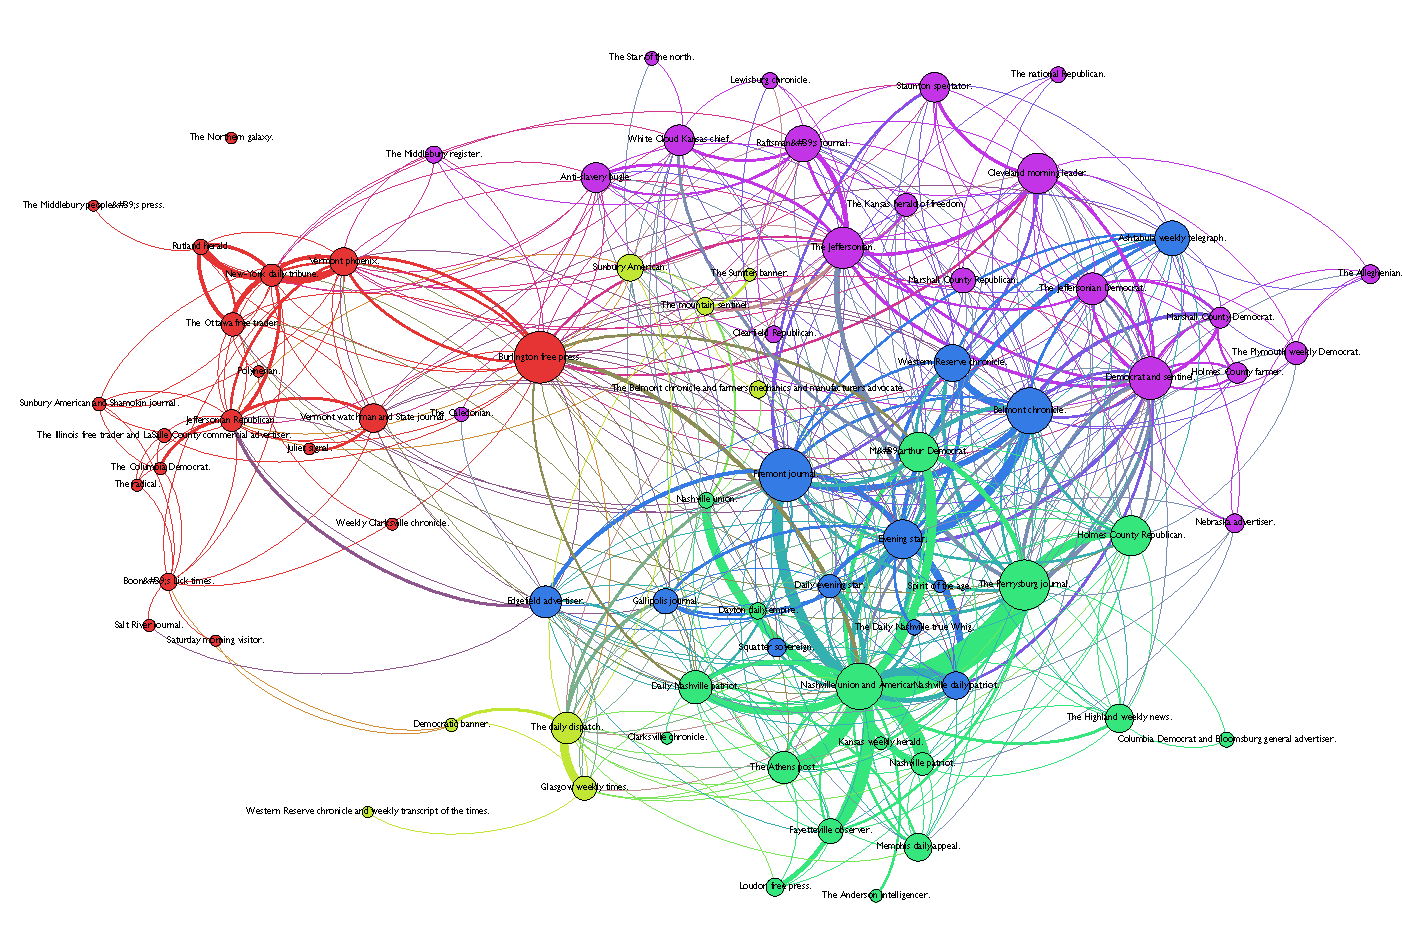
\includegraphics[width=0.5\textwidth]{network}
  \caption{Visualization of the links among newspapers induced by
    shared reprinted texts.  Colors indicate communities derived from
    graph modularity.}
  \label{fig:network}
\end{figure}

\subsection{Reuse Dynamics: Reading Fast and Slow}
\label{sec:fast-slow}

For a reader of today, one of the most striking aspects of 19c
U.S. newspapers is the mixture of what we would recognize as news
items with other genres such as poetry, chapters of novels, jokes, and
morally edifying anecdotes of vague origin.  We explore how different
genres may be distinguished not only by their content but also by the
temporal pattern of their spread.

Some texts are reprinted frequently at first and then become less
popular; others continue to attract interest from newspaper
editors---and presumably readers---for years afterwards.
Figure~\ref{fig:lag-year} shows the median lag time, in log number of
days, between the first observed appearance and later reprints.  The
lag times are plotted by the year of a text's first occurrence.  (We
omit plots for 1856--60 due to boundary effects.)  Most obviously,
there are simply more texts (and more newspapers) as time goes on.  In
many years, there are two peaks in the frequency of lag time, at
around one week and over 3 years.  In 1846--7, for example, there is
an increase in short lag-time, ``fast'' texts, due in part to coverage
of the Mexican-American War.  These fast texts later become more
frequent.  We suspect that the rise of wire services plays a role,
though more research is needed.

Not surprisingly, different kinds of texts travel fast and slow.  We
divided reprinted texts into a fast set, with median lag times under
one year, and a slow set, with median lag times over five years, which
gave approximately equal sets.  We trained a logistic regression model
to predict whether a text would be fast or slow.  Features were all
words in a text's first occurrence that (1) were five characters or
more in length and (2) occurred five or more times in the corpus.  The
year of first occurrence was included as a categorical feature, to
account for the different proportions in fast and slow texts over
time.  The training objective function was regularized with an $L_1$
(Lasso) penalty to achieve a sparse set of predictors
\cite{friedman08:_regul_paths_gener_linear_model_coord_descen}.

Table~\ref{tab:lag-features} shows the top negative (``fast'') and
positive (``slow'') coefficients.  Highly correlated with fast textual
propagation, for example, are terms related to the Mexican-American
War, such as \emph{Texas}, \emph{Mexico}, and [Zachary] \emph{Taylor}.
Also interesting are \emph{government} and \emph{tariff}, \emph{cases}
and \emph{corpse}.  Slow texts focus on \emph{love} and other
affective terms, on \emph{heaven} and interestingly \emph{woman}.  The
year \emph{1840} is also a useful predictor since fewer texts from
that year were fast.  With a random split between training and test,
logistic regression achieved 73\% accuracy on test.  When earlier
years (1840--1849) were used to predict a later one (1850), accuracy
fell to 60\%.  Taking the cross product of year and word features only
slightly diminished overfitting; more analysis of the rhetorical
patterns of different genres should be helpful.  Linear regression on
the log median lag produced similar coefficients but fairly poor
predictive accuracy.

\begin{figure}
  \centering
  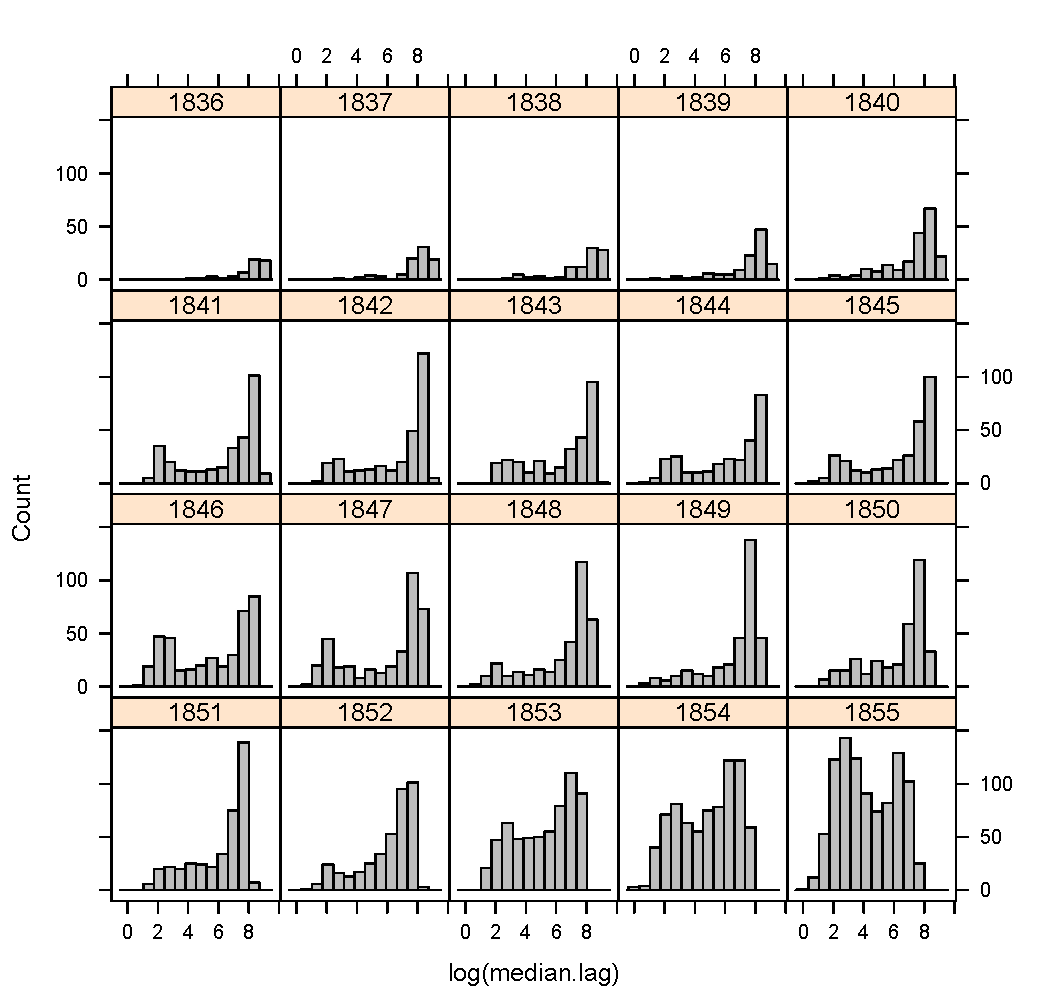
\includegraphics[width=0.5\textwidth]{lag-year}
  \caption{Median lag time, in log days, of reprints
    from first appearance, by year of first appearance.  Many years
    show peaks around 2 ($\approx 1$ week) and 7 ($\approx 3$ years).}
  \label{fig:lag-year}
\end{figure}

\begin{table}
  \small
  \centering
  \caption{Top features from model predicting the lag in
    reprinting.  ``Fast'' texts have a median reprinting time of a
    year or less; ``slow'' texts have a median reprinting time of at
    least five years.}
  \label{tab:lag-features}
  \begin{tabular}{l r|l r}
\multicolumn{2}{c|}{``Fast'' texts} &
\multicolumn{2}{c}{``Slow'' texts} \\ \hline
texas & -0.700 & love & 0.459\\
mexico & -0.692 & young & 0.154\\
pills & -0.672 & earth & 0.138\\
taylor & -0.649 & 1840 & 0.129\\
tariff & -0.534 & awoke & 0.121\\
government & -0.502 & fine & 0.098\\
board & -0.463 & silence & 0.097\\
effect & -0.428 & benevolence & 0.078\\
whig & -0.426 & soul & 0.057\\
mate & -0.418 & sweet & 0.048\\
prices & -0.418 & grant & 0.035\\
goods & -0.416 & hang & 0.033\\
corpse & -0.387 & behold & 0.026\\
cases & -0.383 & bright & 0.025 \\
general & -0.370 & woman & 0.020\\
public & -0.368 & things & 0.020\\
cure & -0.367 & heaven & 0.019\\
%intelligencer & -0.364 & mood & 0.015\\
%army & -0.349 & forever & 0.009\\
%mexican & -0.337 & waiting & 0.001\\
  \end{tabular}
\end{table}

\section{Extrinsic Evaluation}
\label{sec:extrinsic}

While political scientists, historians, and literary scholars will, we
hope, find these techniques useful and perform close reading and
manual analysis on texts of interest, we would like to validate our
results without a costly annotation campaign.  We explore the
correlation of patterns of text reuse with independently acquired
information about newspaper editors.  This idea was inspired by
\cite{margolin13:_why_simil}, who used these techniques to test
rhetorical theories of ``semantic organizing processes'' on a corpus
of congressional statements.

The approach is quite simple: measure the correlation between some
metric of text reuse between actors in a social network and other
features of the network links between those actors.  The metric of
text reuse might be simply the number of exact n-grams shared by the
language of two authors \cite{margolin13:_why_simil}; alternately, it
might be the absolute or relative length of all the aligned passages
shared by two authors or the tree distance between them in a
phylogenetic reconstruction.  To measure the correlation of a text
reuse metric with a single network, we can simply use Pearson's
correlation; for more networks, we can use multivariate regression.
Due to, for instance, autocorrelation among edges arising from a
particular node, we cannot proceed as if the weight of each edge in
the text reuse network can be compared independently to the weight of
the corresponding edges in other networks.  We therefore use
nonparametric permutation tests using the quadratic assignment
procedure (QAP) to resample several networks with the same structure
but different labels and weights.  The QAP achieves this by reordering
the rows and columns of one network's adjacency matrix according to
the same permutation.  The permuted network then has the same
structure---e.g., degree distribution---but should no longer exhibit
the same correlations with the other network(s).  We can run QAP to
generate confidence intervals for both single
\cite{krackhardt87:_qap_partial_test_spurious} and multiple
correlations \cite{dekker07:_sensit_mrqap_tests_collin_autoc_condit}.

\subsection{Network Connections of 19c Reprints}
\label{sec:regress-reprint}

For the antebellum newspaper corpus, we are also interested in how
political affinity correlates with reprinting similar texts.  We have
also added variables for social causes such as temperance, women's
rights, and abolition that---while certainly not orthogonal to
political commitments---might sometimes operate independently.  In
addition, we also added a ``shared state'' variable to account for
shared political and social environments of more limited scope.
Figure~\ref{fig:brown-speech} shows a particularly strong example of a
geographic effect: the statement of the radical abolitionist John
Brown after being condemned to death for attacking a federal arsenal
and attempting to raise a slave rebellion was very unlikely to be
published in the South.

Using information from the Chronicling America cataloguing and from
other newspaper histories, we coded each of the 132 newspapers in the
corpus with these political and social affinities.  We then counted
the number of reprinted passages shared by each pair of
newspapers.  There is not a deterministic relationship between the
number of \emph{pairs} of newspapers sharing an affinity and the
number of \emph{reprints} shared by those papers.  While our
admittedly partial corpus only contains a single pair of avowedly
abolitionist papers---a radical position at the time---those two
papers shared articles 306 times, compared for instance to the 71
stories shared among the 6 pairs of ``nativist'' papers.

Table~\ref{tab:newspaper-regression} shows that geographic proximity
had by far the strongest correlation with (log) reprinting counts.
Interestingly, the only political affinity to show as strong a
correlation was the Republican party, which in this period had just
been organized and, one might suppose, was trying to control its
``message''.  The Republicans were more geographically concentrated in
any case, compared to the sectionally more diffuse Democrats.  Another
counterexample is the Whigs, the party from which the new Republican
party drew many of its members, which also has a slight negative
effect on reprinting.  The only other large coefficients are in the
complete model for smaller movements such as nativism and abolition.
It is interesting to speculate about whether the speed or faithfulness
of reprinting---as opposed to the volume---might be correlated with
more of these variables.

\begin{figure}
  \centering
  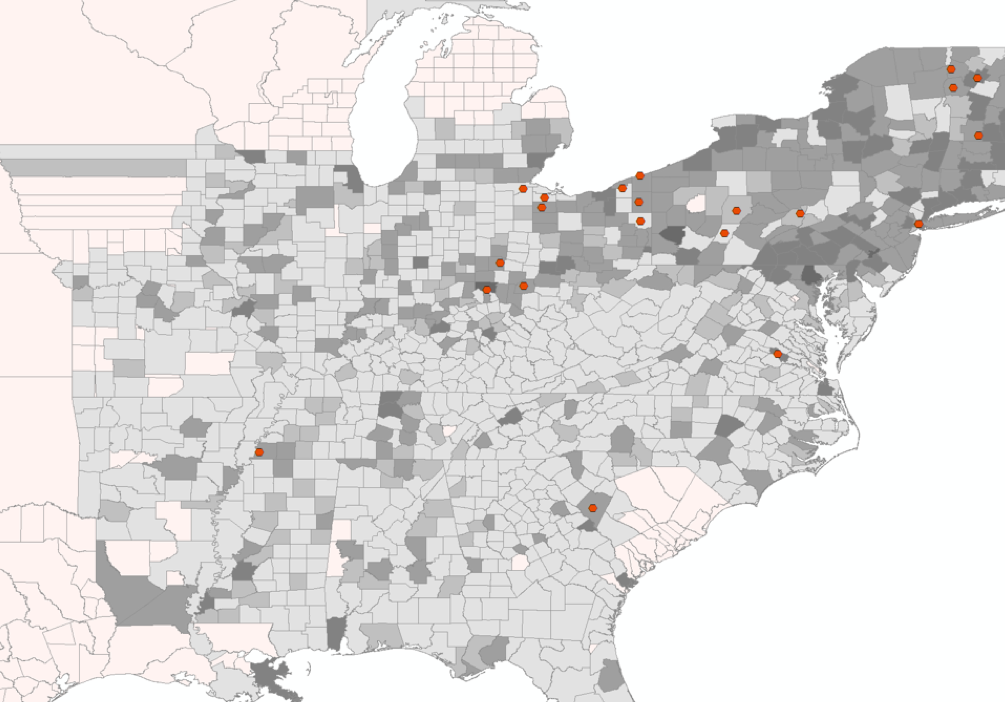
\includegraphics[width=0.5\textwidth]{brown-speech}
  \caption{Reprints of John Brown's 1859 speech at his
    sentencing. Counties are shaded with historical population data,
    where available.  Even taking population differences into account,
    few newspapers in the South printed the abolitionist's statement.}
  \label{fig:brown-speech}
\end{figure}

\begin{table*}
  \centering
  \begin{tabular}{rrrlll}
    newspaper & \multicolumn{2}{c}{pairs of} & \multicolumn{3}{c}{regression w/pairs} \\
    affinity & papers & reprints & $\ge 1$ & $\ge 10$ & $\ge 100$ \\ \hline
    Republican & 1176 & 134,302 & 0.74*** & 0.73* & 0.72*** \\
    Whig & 1176 & 91,139 & -0.35 & -0.34 & -0.35 \\
    Democrat & 1081 & 62,609 & -0.08 & -0.09 & -0.07 \\
    same state & 672 & 103,057 & 1.12*** & 1.11*** & 1.13*** \\
    anti-secession & 435 & 22,009 & -0.58* & -0.58 & -0.60 \\
    anti-slavery & 231 & 12,742 & -0.65 & -0.64 & -0.60 \\
    pro-slavery & 120 & 11,040 & -0.35 & -0.35 & -0.27 \\
    Free-State & 15 & 1,194 & 0.80 & 0.80 & \\
    Constitutional Union & 15 & 1,070 & -0.21 & -0.21 & \\
    pro-secession & 15 & 529 & 0.11 & 0.11 & \\
    Free Soil & 10 & 1,936 & -0.42 & -0.42 & \\
    Copperhead & 10 & 797 & 1.53 & 1.54 & \\
    temperance & 6 & 560 & 0.65 & & \\
    independent & 6 & 186 & -0.22 & & \\
    nativist & 6 & 71 & -1.93* & & \\
    women's rights & 3 & 721 & 1.91 & & \\
    abolitionist & 1 & 306 & 3.49** & & \\
    Know-Nothing & 1 & 25 & 1.33 & & \\
    Mormon & 1 & 3 & -1.13 & & \\ \hline
    R-squared & -- & -- & .065 & .063 & .062 \\    
  \end{tabular}
  \caption{Correlations between shared reprints between 19c newspapers and political and other affinities.  While many Whig papers became Republican, they do not completely overlap in our dataset; the identical number of pairs is coincidental.}
  \label{tab:newspaper-regression}
\end{table*}

\section{Conclusions}
\label{sec:conclusions}

We have described efficient algorithms that exploit shingling,
space-efficient hashed indexing, and local alignment to detect
clusters of passages reprinted within large collections of OCR'd texts
without a priori knowledge of which texts were repeated.  Applied to
collections of 19c newspapers and Congressional bills, these
techniques allow us to explore how ideas spread, which ideas spread,
and which subgroups shared ideas.

\section*{Acknowledgements}

This work was supported in part by NEH Digital Humanities Start-Up
Grant \#HD-51728-13, by a grant from the Andrew W. Mellon Foundation's
Scholarly Communications and Information Technology program, by
Northeastern University's Tier 1 grant program for interdisciplinary
research, and by the NUlab for Texts, Maps, and Networks.  Any views,
findings, conclusions, or recommendations expressed do not necessarily
reflect those of the NEH or Mellon.

\bibliographystyle{plainnat}
\bibliography{confnames,infect}

\end{document}


